The CPPN/NEAT architecture is at the forefront of the facial deformation discovery process. The architecture takes 
advantage of developed software suites most notably HyperNEAT C++ \cite{jasongauci}. HyperNEAT C++ is a complete
version of NEAT, CPPN/NEAT and HyperNEAT that was suited to prove the validity of the HyperNEAT platform. 
Extensions to this original program had to be made in order to tailor it to the field of facial deformations. 
HyperNEAT C++ was extended with the Python programming language in order to create easier accessibility to the
underlying algorithmic process. The architecture presented in this paper is simple and allows for quick 
evaluation of image novelty by the user. The simple architecture \ref{fig:paper:architecture} allows for recursive 
processing of information in order to process not only static images but videos and allows expansion to
include more complex deformations including non Human faces.

\begin{figure}
    \centering
    \label{fig:paper:interface}
    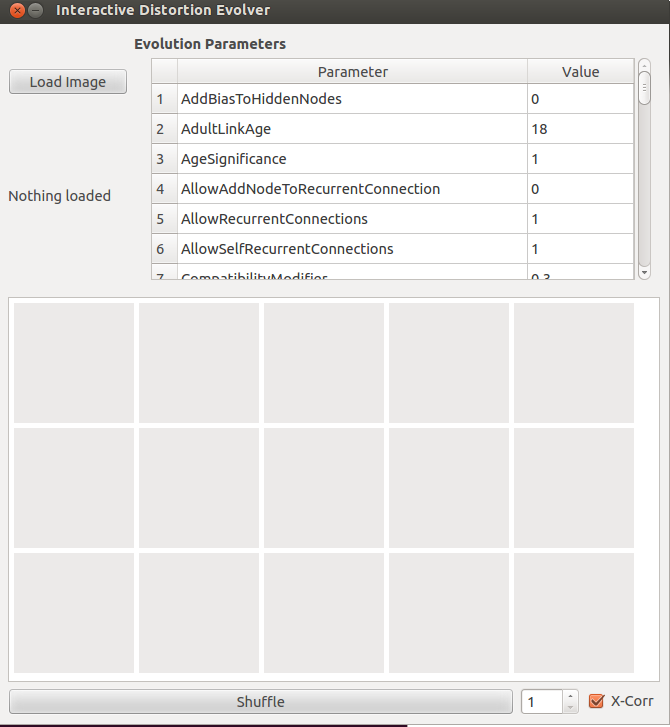
\includegraphics[width=0.4\textwidth]{../../rec/paper/interface.png}
    \caption{User interface for interactive evolution.}
\end{figure}

\begin{figure*}
    \centering
    \label{fig:paper:architecture}
    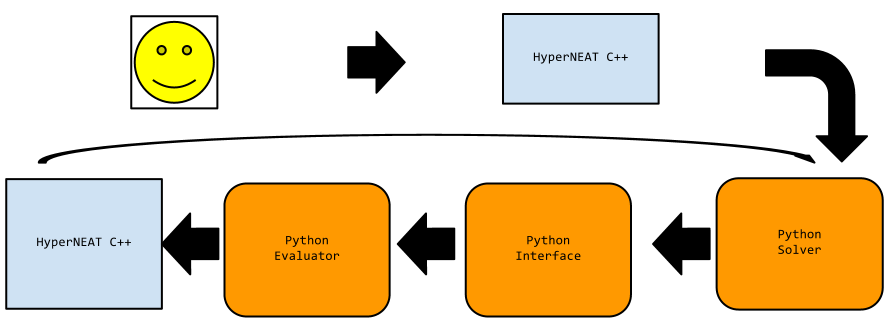
\includegraphics[width=0.6\textwidth]{../../rec/paper/architecture.png}
    \caption{Facial deformations architecture.}
\end{figure*}

The major issues with the architecture became obvious when running, the most glaring issue was that of user fatigue.
Cited in many major publications user fatigue is the anomaly that occurs when users are presented with a long search process
\cite{secretan2008picbreeder} \cite{li2009innovative}. Due to the constructive nature of genetic art in that each part or symmetry
is discovered in an orderly process and innovative structures are seldom seen by the user. Users frequently expect the innovative
images to be produced immediately, but this is inhibited by the expansive search space and no knowledge of what constitutes an 
mathematically interesting image. This problem is further exacerbated by the presence of noise in the genotype to phenotype 
representation. This noise takes the form of large changes to the underlying neural network structure producing relatively small
changes in the images. These small changes take the form of rotational and translational image transformations and represent the
phenotype of the large change in the genotype. It was discovered that these jumps occur more at lower complexity levels than at
larger levels and occur with a relative frequency. The combination of user fatigue, nonlinear mapping, and low complexity leads to
uninteresting images being produced by the algorithmic process. It is theorized that these issues would be solved given more users
with programs such as PicBreeder, as the process can be parallelized and utilize user histories to solve not only the fatigue issue
but also the complexity issues \cite{secretan2008picbreeder}.

Unable to acquire more users these issues had to be addressed in order for new novel structures to be discovered by the algorithmic
process. Using the insight that the novel structures represent something that has not been discovered before a novelty like search
algorithm can be implemented \cite{lehman2010efficiently}. The biggest hurdle is to discover a function of novelty of an image, this
was discovered by accident through observation. Using a image histogram a simple entropy calculation can be performed. This histogram
is then averaged over the mean and standard deviation of all images in the historical novelty record to discover the offset the image
represents. A simple threshold of a correlation matrix is then used to determine if the image is novel or not and whether to present this image to the user.
This threshold is troublesome as small changes in it can create large differences in the number of novel images selected to be presented
to the user. To further solve this problem a W3C luminance calculation is performed which transforms the red,green,blue image which
varies from [0,255] to luminosity (contrast) values between [1,21] this smaller variation value allows less emphasis to be placed
on threshold placement \cite{W3C}.Image entropic value estimation though does not solve the rotation issues present, but through 
empirical analysis it lessens the impact, due to usage of an offset rather then a direct value evaluation. Novelty search in combination
with image entropy metric allows a solution to user fatigue to become present as non-novel images are greatly reduced. Novelty search
solves the user fatigue issue but does not solve the complexification issue that remains. 

Even with the addition of novelty search the initial search process starts out very slow as the network builds complexity. To solve this 
a shuffle and randomization ability was created to boost the algorithm to a higher dimensional space quickly without user interaction.
A Gaussian distribution is used with which new random evaluation values are given to novel images in the search space. The Gaussian
distribution was found to be key as the algorithm would become confused if on one generation an image became very highly valued and the next
was considered junk due to the randomness. Having a smooth random fitness function for the population members allows each species to equally
have a chance to become complex while stopping confusion as the fitness gradually levels off with time rather than be subject to computational
randomness. The complexification of these initial functions allows for user fatigue to be further curtailed and the novel facial 
deformations to be discovered by the user.